\subsection{Visitor}
\label{visitor}

\textbf{Scopo}: Comportamentale \\
\textbf{Raggio d'azione}: Oggetti

\paragraph{Definizione} Il pattern Visitor rappresenta un’operazione da eseguire sugli oggetti di una struttura e consente di definire nuove operazioni senza modificare le classi degli oggetti su cui opera (vantaggioso).

\paragraph{Vantaggi} Da la possibilità di aggiungere dinamicamente delle nuove operazioni, senza interrompere l'esecuzione perchè le operazioni vengono integrate in degli oggetti.

\begin{figure}[H]
    \centering
    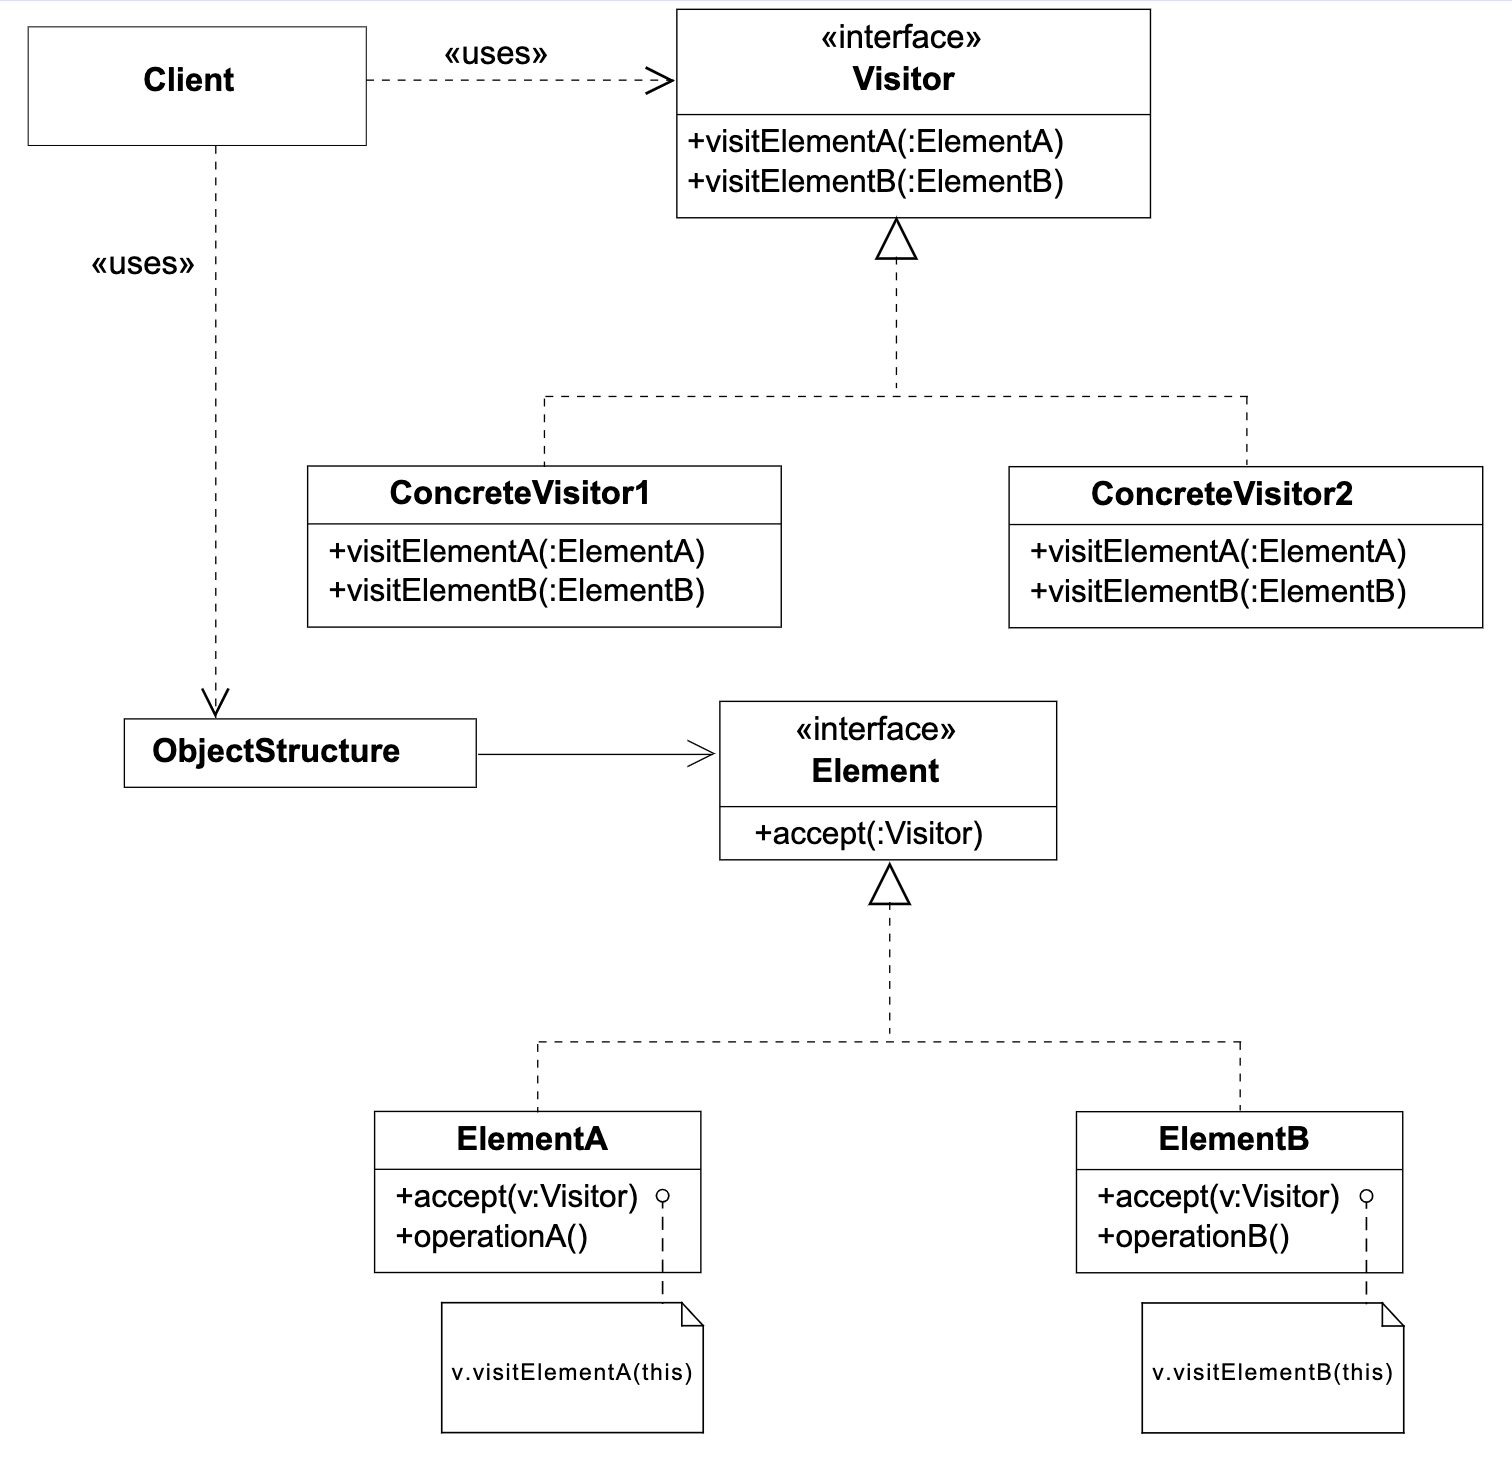
\includegraphics[width=1\linewidth]{assets/pattern/visitor/visitor-struttura.png}
    \caption{Struttura del pattern}
\end{figure}

\newpage

\paragraph{Struttura e Interazioni} Il pattern è composto da:
\begin{itemize}
    \item \textbf{Visitor}: dichiara un metodo di visita per ogni classe concreta della struttura, il nome e la firma del metodo identificano la classe che invia la richiesta di visita al visitor in modo che il visitor possa identificare la classe dell’elemento che sta per visitare 
    \item \textbf{ConcreteVisitor}: implementa i metodi definiti da Visitor. Ogni metodo implementa un frammento dell’algoritmo definito per la struttura. In più fornisce il contesto per l’algoritmo e memorizza il suo stato locale che accumula durante la visita della struttura. 
    \item \textbf{Element}: definisce il metodo \textit{accept()} che riceve un Visitor.
    \item \textbf{ConcreteElements}: implementano il metodo \textit{accept()} che riceve un Visitor.
    \item \textbf{ObjectStructure}: può enumerare gli elementi che la costituiscono. può essere realizzata come un Composite o come una collezione di elementi.
\end{itemize}

\begin{figure}[H]
    \centering
    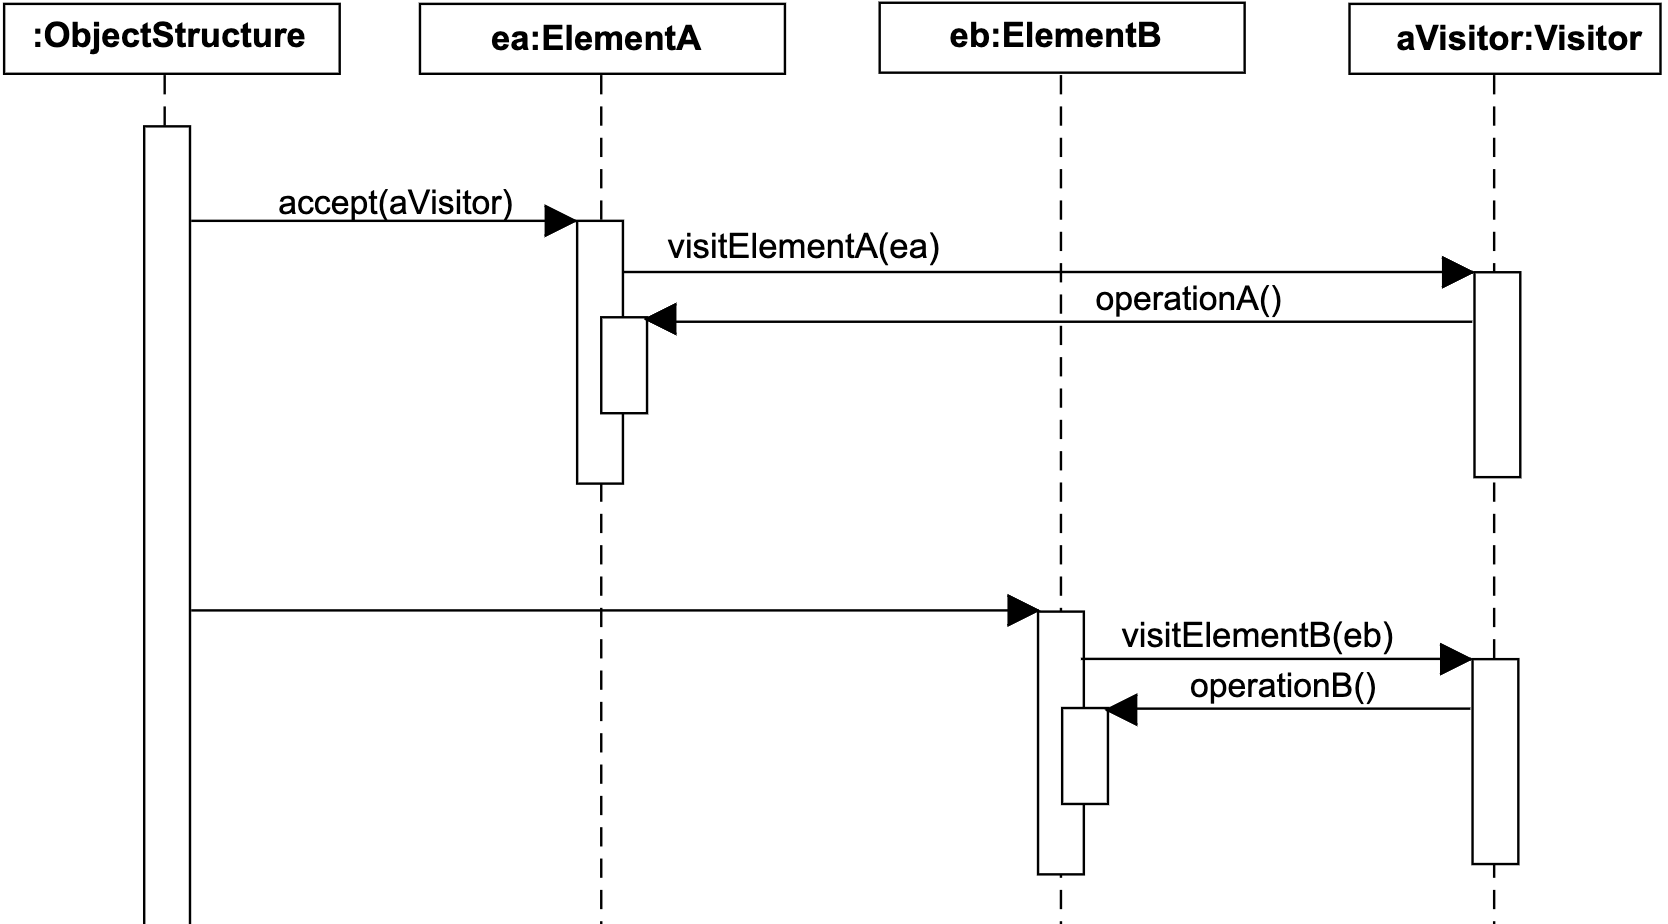
\includegraphics[width=1\linewidth]{assets/pattern/visitor/visitor-sequence.png}
    \caption{Sequence Diagram del pattern Visitor}
\end{figure}

\paragraph{Correlazioni} Il pattern Visitor può essere utilizzato per applicare un'operazione su una struttura di oggetti implementata attraverso il pattern Composite (\ref{composite}) oppure per eseguire l'effettiva interpretazione di un'espressione (Interpreter, \ref{interpreter}).


\newpage